%\begin{center}
%	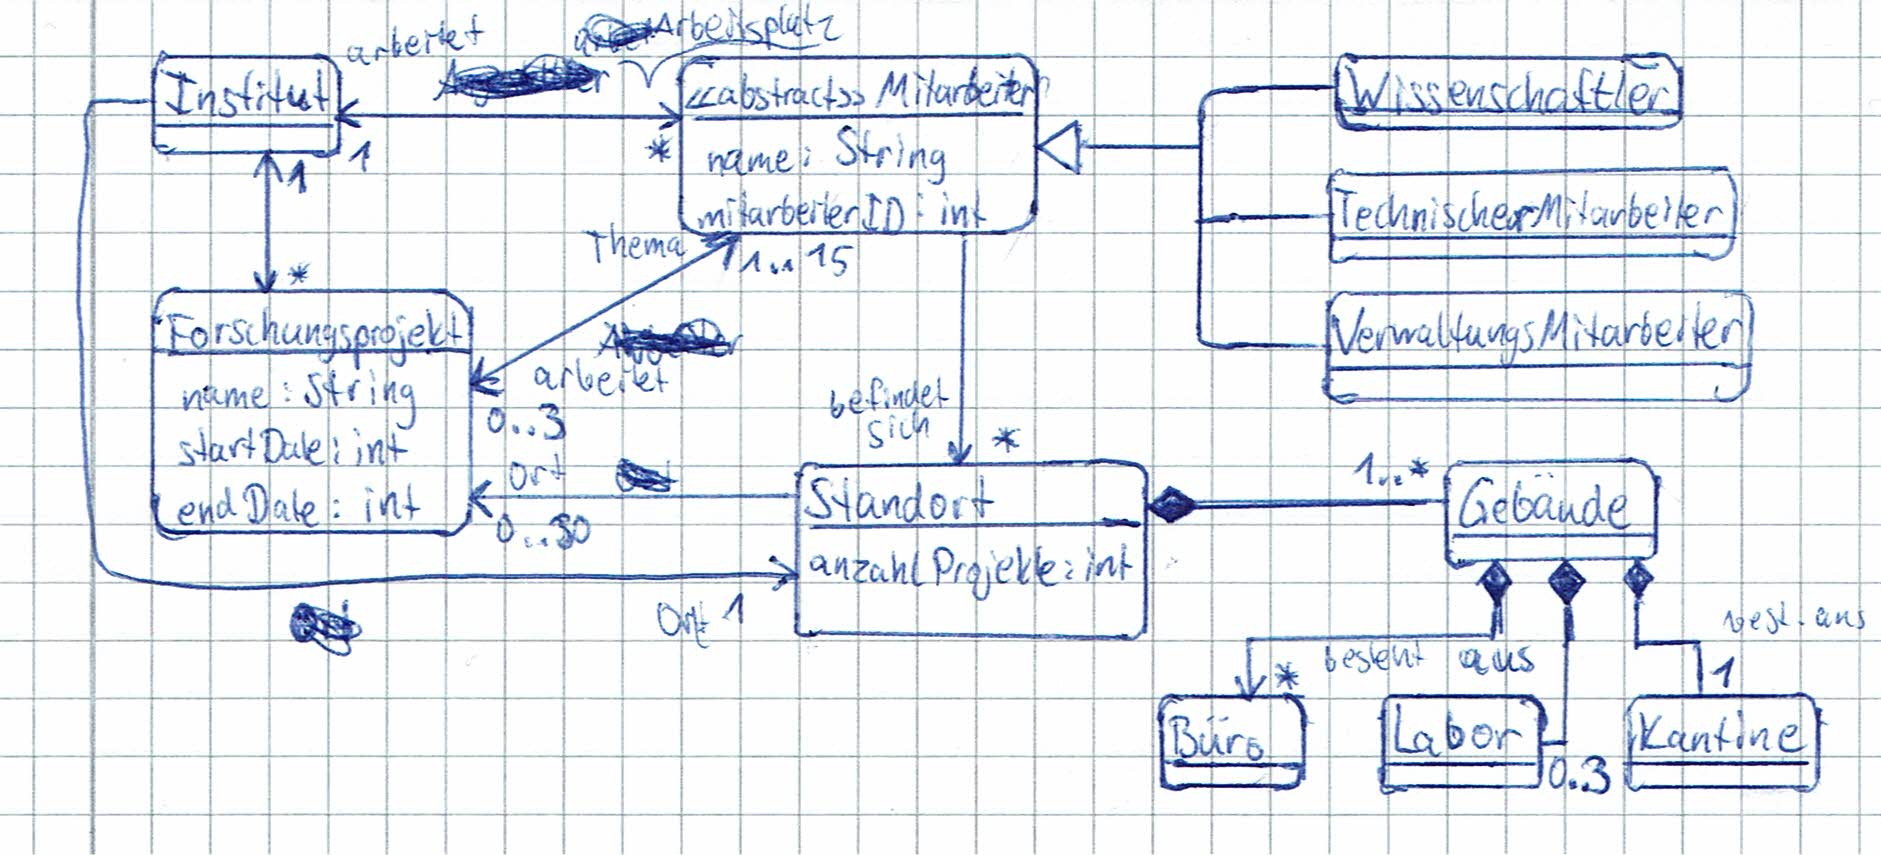
\includegraphics[scale=0.8]{51_TODO.jpg}
%\end{center}

\begin{tikzpicture}

	\umlsimpleclass[anchor=north west]{Institut}{}{}
	\umlclass[anchor=south west,y=-6]{Forschungsprojekt}
		{name : String \\ startDate: int \\ endDate : int}{}
	\umlclass[x=5,anchor=north,type=abstrakt]
		{Mitarbeiter}{name : String \\ mitarbeiterID : int}{}
	\umlsimpleclass[x=8,y=0,anchor=north west]{Wissenschaftler}
	\umlsimpleclass[x=8,y=-1,anchor=north west]{TechnischerMitarbeiter}
	\umlsimpleclass[x=8,y=-2,anchor=north west]{VerwaltungsMitarbeiter}
	\umlclass[x=7.5,y=-6]{Standort}{anzahlProjekte: int}{}
	\umlclass[x=12,y=-6]{Gebäude}{}{}
	\umlsimpleclass[x=9,y=-9,anchor=east]{Büro}
	\umlsimpleclass[x=10,y=-9]{Labor}
	\umlsimpleclass[x=11,y=-9,anchor=west]{Kantine}
	
	\umluniassoc[anchor2=153,mult=*,pos=0.85]{Institut}{Mitarbeiter}
	\umluniassoc[anchor1=153,mult=1,align=right,pos=0.6]{Mitarbeiter}{Institut}

	\umlHVHinherit[anchor2=20]{Wissenschaftler}{Mitarbeiter}
	\umlHVHinherit[anchor2=0]{TechnischerMitarbeiter}{Mitarbeiter}
	\umlHVHinherit[anchor2=-20]{VerwaltungsMitarbeiter}{Mitarbeiter}

	\umluniassoc[anchor1=-42,anchor2=140,arg=befindet sich,mult=*,pos=0.8]
		{Mitarbeiter}{Standort}
	
	\umlcompo[mult=1..*]{Standort}{Gebäude}
	\umlVHVunicompo[arg1=besteht aus,mult2=*,pos2=2.9,pos1=1.2,anchor1=-120,
		align1=right,weight=0.5]{Gebäude}{Büro}
	\umlVHVunicompo[arg1=besteht aus,mult2=0..3,pos2=2.7,pos1=1.2,anchor1=-90,
		align1=right,weight=0.65]{Gebäude}{Labor}
	\umlVHVunicompo[arg1=besteht aus,mult2=1,pos2=2.6,pos1=0.8,anchor1=-60,
		weight=0.7]{Gebäude}{Kantine}

	\umlHVHuniassoc[mult2=1,arg2=Ort,anchor1=180,weight=-0.2,anchor2=200,
		pos2=2.9,align2=right]{Institut}{Standort}
	
	\umluniassoc[mult2=0..30,arg2=Ort,anchor1=165,anchor2=-22,align2=left,pos2=0.9]
		{Standort}{Forschungsprojekt}

	\umlVHuniassoc[mult2=0..3,arg2=arbeitet,anchor1=-70,anchor2=10,pos=1.9,align=left]
		{Mitarbeiter}{Forschungsprojekt}
	\umlHVuniassoc[mult2=1..15,arg2=Thema,anchor2=-70,anchor1=10,pos=1.9]
		{Forschungsprojekt}{Mitarbeiter}
	
	\umluniassoc[mult2=*,anchor1=-60,anchor2=119,align=left,pos=0.8]
		{Institut}{Forschungsprojekt}
	\umluniassoc[mult2=*,anchor2=-60,anchor1=119,pos=1]
		{Forschungsprojekt}{Institut}

\end{tikzpicture}
